\documentclass[11pt, english]{beamer}
\usepackage{mathptmx}
\renewcommand{\sfdefault}{lmss}
\renewcommand{\familydefault}{\sfdefault}
\usepackage[T1]{fontenc}
\usepackage[latin9]{inputenc}
\usepackage{amsmath}
\usepackage{amssymb}
\usepackage{graphicx}
\PassOptionsToPackage{normalem}{ulem}
\usepackage{ulem}
\usepackage{caption}
\captionsetup{labelformat=empty}
\usepackage{bbm}
\usepackage{upgreek}
\usepackage{graphicx}
\setbeamertemplate{section in toc}[sections numbered]
\makeatletter
\usepackage{caption}
\captionsetup[table]{skip=10pt}
%%%%%%%%%%%%%%%%%%%%%%%%%%%%%% Textclass specific LaTeX commands.
% this default might be overridden by plain title style
\newcommand{\makebeamertitle}{\frame{\maketitle}}%
% (ERT) argument for the TOC
\AtBeginDocument{%
\let\origtableofcontents=\tableofcontents \def\tableofcontents{\@ifnextchar[{\origtableofcontents}{\gobbletableofcontents}} \def\gobbletableofcontents#1{\origtableofcontents} }

\setbeamersize{text margin left=.8em, text margin right=1em}
\newenvironment{wideitemize}{\itemize
\addtolength{\itemsep}{10pt}}{\enditemize}
\newenvironment{wideitemizeshort}{\itemize}{\enditemize}

%%%%%%%%%%%%%%%%%%%%%%%%%%%%%% User specified LaTeX commands.
%\documentclass[presentation]{beamer}

\def\Tiny{\fontsize{7pt}{8pt}\selectfont}
\def\Normal{\fontsize{8pt}{10pt}\selectfont}

\usetheme{Madrid}
\usecolortheme{lily}
%\setbeamercovered{transparent}
\useinnertheme{rounded}

\setbeamertemplate{footline}{
	\hfill\Normal{\insertframenumber/\inserttotalframenumber}
}
%\setbeamertemplate{footline}{}

\setbeamertemplate{navigation symbols}{}

\newenvironment{changemargin}[2]{%
\begin{list}{}{%
\setlength{\topsep}{0pt}%
\setlength{\leftmargin}{#1}%
\setlength{\rightmargin}{#2}%
\setlength{\listparindent}{\parindent}%
\setlength{\itemindent}{\parindent}%
\setlength{\parsep}{\parskip}%
}%
\item[]}{\end{list}}

\setbeamertemplate{footline}{\hfill\insertframenumber/\inserttotalframenumber}
\setbeamertemplate{navigation symbols}{}

%\usepackage{times}  % fonts are up to you
\usepackage{graphicx}
%\usepackage{graphics}
\usepackage{epsfig}
\usepackage{bm}
\usepackage{epsf}
\usepackage{float}
\usepackage[final]{pdfpages}
\usepackage{multirow}
\usepackage{colortbl}
\usepackage{xkeyval}
%\usepackage{sgame}
%\usepackage{pst-node}
\usepackage{listings}
\usepackage{ifthen}
%\usepackage{hyperref}
\usepackage{tikz}

%\usepackage{times}  % fonts are up to you
%\usepackage{graphicx}
%\usepackage{graphics}
\usepackage{epsfig, bm, epsf, float}
\usepackage[final]{pdfpages}
\usepackage{xcolor, multirow, colortbl}
\usepackage{xkeyval}
\usepackage{verbatim}
%\usepackage{sgame}
%\usepackage{pst-node}
\usepackage{listings}
%\usepackage{handoutWithNotes}
%\pgfpagesuselayout{3 on 1 with notes}[letterpaper,border shrink=5mm]
%\pgfpagesuselayout{2 on 1 with notes landscape}[letterpaper,border shrink=5mm]
\usepackage{setspace}
\usepackage{ragged2e}

\setbeamersize{
	text margin left=1em,
	text margin right=1em
} % CambridgeUS spacing if you use default instead

%\pdfmapfile{+sansmathaccent.map}

% Table formatting
\usepackage{booktabs}

% Decimal align
\usepackage{dcolumn}
\newcolumntype{d}[0]{D{.}{.}{5}}

\newcommand{\independent}{\protect\mathpalette{\protect\independenT}{\perp}}
\def\independenT#1#2{\mathrel{\rlap{$#1#2$}\mkern2mu{#1#2}}}

\global\long\def\expec#1{\mathbb{E}\left[#1\right]}
\global\long\def\var#1{\mathrm{Var}\left[#1\right]}
\global\long\def\cov#1{\mathrm{Cov}\left[#1\right]}
\global\long\def\prob#1{\mathrm{Prob}\left[#1\right]}
\global\long\def\one{\mathbf{1}}
\global\long\def\diag{\operatorname{diag}}
\global\long\def\expe#1#2{\mathbb{E}_{#1}\left[#2\right]}
\DeclareMathOperator*{\plim}{\text{plim}}

%\usefonttheme[onlymath]{serif}

\usepackage{appendixnumberbeamer}
\renewcommand{\thefootnote}{}

\setbeamertemplate{footline}{
	\leavevmode %
	%   \hbox{%
	%      \begin{beamercolorbox}[wd=\paperwidth,ht=2.25ex,dp=1ex,right]{date in head/foot}%
	%\usebeamerfont{date in head/foot}\insertshortdate{}\hspace*{2em}%
	\hfill
	%turning the next line into a comment, erases the frame numbers
	\insertframenumber{}\hspace*{2ex}\vspace{1ex}

	%    \end{beamercolorbox}}%
}

\definecolor{blue}{RGB}{0, 0, 210}
\definecolor{red}{RGB}{170, 0, 0}

\makeatother

\usepackage[english]{babel}

%\mode<handout>{
%\setbeamercolor{background canvas}{bg=black!5}
%\usepackage{pgfpages}
%\pgfpagesuselayout{2 on 1}[a4paper,border shrink=5mm]
%\pgfpagesuselayout{4 on 1}[a4paper,border shrink=5mm,landscape]
%}
%\newcommand{\opause}{\pause{}}

\usepackage{tikz}
\newcommand*{\circled}[1]{\tikz[baseline=(char.base)]{ \node[circle,ball color=structure.fg,
shade, color=white,inner sep=1.2pt] (char) {\tiny #1};}}

\makeatletter
\let\save@measuring@true\measuring@true
\def\measuring@true{%
\save@measuring@true \def\beamer@sortzero##1{\beamer@ifnextcharospec{\beamer@sortzeroread{##1}}{}}%
\def\beamer@sortzeroread##1<##2>{}%
\def\beamer@finalnospec{}%
}
\makeatother

\begin{document}
	%% Title slide
	\begin{frame}[noframenumbering]{}
		\vspace{0.5cm}
		\title[]{Day 1: Identification by Design}
		\author{Peter Hull}
		\date{Design-Based Regression Inference \\
		Spring 2024}
		\titlepage {\small{}\ }
		\thispagestyle{empty}
		\vspace{-30pt}
	\end{frame}

	\begin{frame}{The Design of This Course}
		\begin{itemize}
			\item This is a three-day intensive in design-based causal inference
				\smallskip
				\begin{itemize}
					\item Far from comprehensive: will focus on core concepts with
						regression/IV
						\smallskip

					\item Emphasis will be on practical lessons for applied work
						\smallskip

					\item I will assume you all have a solid foundation in the basics of causal
						inference (e.g. Scott's intro courses)
				\end{itemize}
				\bigskip
				\pause{}

			\item 6-7 hours of lecture, two 30-minute coding demonstrations
				\smallskip
				\begin{itemize}
					\item Please ask questions in the Discord chat!
						\smallskip

					\item I will try to stick to the schedule but may improvise slightly
						\smallskip

					\item Code assignments will be ``take home,'' w/solutions the
						following class
				\end{itemize}
				\bigskip
				\pause{}

			\item Feedback/follow-up: \emph{peter\_hull@brown.edu}
		\end{itemize}
	\end{frame}

	\begin{frame}{Course Schedule}
		\begin{center}
			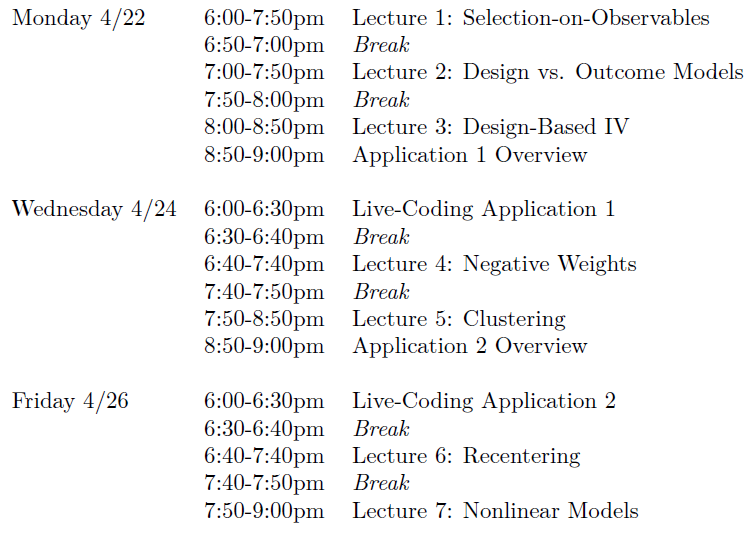
\includegraphics[width=0.85\textwidth]{figures/schedule.png}
		\end{center}
	\end{frame}

	\begin{frame}{The Design \emph{in} This Course}
		\begin{itemize}
			\item Design-based methods use knowledge on the assignment process of as-if-randomly
				assigned shocks to estimate causal effects
				\smallskip
				\begin{itemize}
					\item Mimic analysis of ``true'' experiments, w/known randomization
						protocol
						\smallskip

					\item Contrasts with identification strategies that model untreated potential
						outcomes (e.g. parallel trends) without appealing to randomization
				\end{itemize}
				\bigskip
				\pause{}

			\item Design-based methods have several practical advantages:
				\smallskip
				\begin{itemize}
					\item A large class of robust estimators, which work without
						restricting how unobservables (e.g. potential outcomes) relate to observables
						\smallskip
						\pause{}

					\item Robust regression/IV estimation, avoiding ``negative weight''
						issues
						\smallskip
						\pause{}

					\item Clear criteria for how to pick controls and cluster standard errors
						\smallskip
						\pause{}

					\item Clear(er) role of nonlinear/structural models as extrapolation
						devices
				\end{itemize}
				\bigskip
				\pause{}

			\item We'll get into all of this over the next few days, building up
				slowly...
		\end{itemize}
	\end{frame}

	\begin{frame}{Outline}
		1. Selection on Observables
		\vspace{0.8cm}

		2. Design vs. Outcome Models
		\vspace{0.8cm}

		3. Design-Based IV
	\end{frame}

	\begin{frame}{The Simplest Experimental Story}
		\begin{itemize}
			\item Throughout today, we'll consider the goal of estimating parameter
				$\beta$ in the constant-effects causal model
				\begin{align*}
					y_{i} = \beta x_{i} + \varepsilon_{i}
				\end{align*}
				Here $y_{i}$ and $x_{i}$ are the observed outcome and treatment, while $\varepsilon
				_{i}$ is an unobserved untreated potential outcome
				\smallskip
				\pause{}
				\begin{itemize}
					\item On Wednesday: heterogeneous effects / multiple treatments
				\end{itemize}
				\medskip
				\pause{}

			\item Suppose $x_{i}$ is generated by an experiment:
				$x_{i}\mid \varepsilon \stackrel{iid}{\sim}G$ for some $G$
				\smallskip
				\pause{}
				\begin{itemize}
					\item Treatment is random, so knowing $\varepsilon_{i}$ doesn't help
						you predict it
						\smallskip

					\item This means $0=Cov(x_{i},\varepsilon_{i})\pause{}=Cov(x_{i},y_{i}-
						\beta x_{i})\pause{}=Cov(x_{i},y_{i})-\beta Var(x_{i})$
						\smallskip
						\pause{}

					\item[$\Rightarrow$] $\beta=Cov(x_{i},y_{i})/Var(x_{i})$, which is the
						population slope coefficient from regressing $y_{i}$ on $x_{i}$ (i.e.
						$\beta$ is identified by regression)
						\smallskip
						\pause{}

					\item[$\Rightarrow$] We can estimate $\beta$ by a sample (OLS) regression
						of $y_{i}$ on $x_{i}$
				\end{itemize}
		\end{itemize}
	\end{frame}

	\begin{frame}{Econometrics: The ``Big Picture''}
		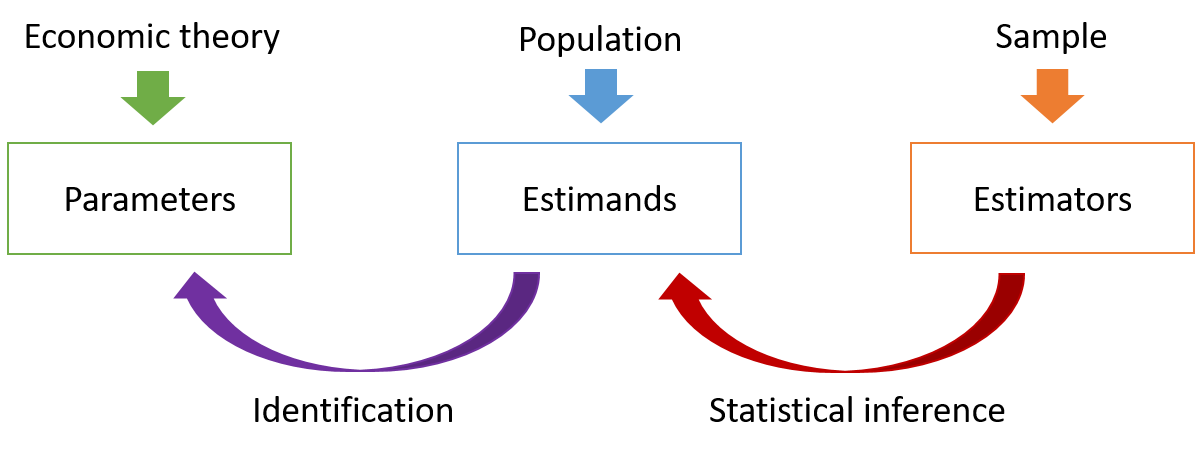
\includegraphics[width=1\textwidth]{figures/BigPicture.png}
		\medskip

		\begin{center}
			Always good to remember which part of the diagram you're working on!
		\end{center}
	\end{frame}

	\begin{frame}{Stratified Randomization}
		\begin{itemize}
			\item Now consider a (slightly) more complicated experimental design:
				$x_{i}\mid w, \varepsilon \stackrel{iid}{\sim}G(w_{i})$ where
				$w_{i}=\{1,2,\dots,K\}$ indexes some strata
				\smallskip
				\pause{}
				\begin{itemize}
					\item E.g. treatment is more available/rationed in across waves or
						cites\pause{}
				\end{itemize}
				\medskip

			\item Consider regressing $y_{i}$ on $x_{i}$, controlling for strata FE, $w
				_{ik}=\mathbf{1}[w_{i}=k]$
				\smallskip
				\pause{}
				\begin{itemize}
					\item By the Frisch-Waugh-Lovell theorem, equivalent to the regression
						of $y_{i}$ on $\tilde{x}_{i}$: the residuals from regressing $x_{i}$
						on the FE
						\smallskip
						\pause{}

					\item But notice since the auxiliary model is \emph{saturated}, $\tilde
						{x}_{i}=x_{i}-E[x_{i}\mid w_{i}]$
						\smallskip
						\pause{}

					\item Hence, the regression gives:
						\vspace{-0.1cm}
						\begin{align*}
							\frac{Cov(\tilde{x}_{i},y_{i})}{Var(\tilde{x}_{i})}=\frac{Cov(\tilde{x}_{i},\beta x_{i}+\varepsilon_{i})}{Var(\tilde{x}_{i})}=\beta +\frac{Cov(\tilde{x}_{i},\varepsilon_{i})}{Var(\tilde{x}_{i})}
						\end{align*}\pause{}

					\item Moreover, by the LIE and conditional random assignment:
						\begin{align*}
							Cov(\tilde{x}_{i},\varepsilon_{i})=E[(x_{i}-E[x_{i}\mid w_{i}])\varepsilon_{i}]=E[(E[x_{i}\mid w,\varepsilon]-E[x_{i}\mid w_{i}])\varepsilon_{i}]=0
						\end{align*}
						\vspace{-0.5cm}
						\pause{}

					\item Thus, the strata-controlled regression identifies the parameter
						$\beta$
				\end{itemize}
		\end{itemize}
	\end{frame}

	\begin{frame}{Selection on Observables}
		\begin{itemize}
			\item Design-based regressions in observational data appeal to such experimental
				ideals:
				\smallskip
				\begin{enumerate}
					\item Claim $x_{i}$ is as-good-as-randomly assigned conditional on some
						$w_{i}$: formally, $x_{i} \mid w,\varepsilon \sim G(w_{i})$
						\smallskip
						\pause{}

					\item Control flexibly for $w_{i}$, such that the auxiliary regression
						of $x_{i}$ on this estimates $E[x_{i}\mid w_{i}]$ ($\implies$ the controlled
						reg uses $\tilde{x}_{i}=x_{i}-E[x_{i}\mid w_{i}]$)
				\end{enumerate}
				\bigskip
				\pause{}

			\item Two steps to make such appeals convincing:
				\smallskip
				\pause{}
				\begin{enumerate}
					\item Tell a clear \emph{ex ante} story about where the
						$x_{i}\mid w_{i}$ variation comes from and why it is unlikely to be
						correlated with $\varepsilon_{i}$
						\smallskip
						\pause{}

					\item Use \emph{ex post} balance tests to check that $x_{i}$ is not
						correlated, conditional on $w_{i}$, with other observables that may
						proxy for $\varepsilon_{i}$
				\end{enumerate}
		\end{itemize}
	\end{frame}

	\begin{frame}{Example: Dale and Krueger (2002)}
		\begin{itemize}
			\item D\&K estimate effects of attending a more selective college (e.g., a
				private school) on adult earnings
				\smallskip
				\begin{itemize}
					\item They have data on schooling and earnings, as well as information
						on which colleges individuals applied to and got into
				\end{itemize}
				\bigskip
				\pause{}

			\item \emph{Ex ante} selection-on-observables story:
				\smallskip
				\begin{itemize}
					\item Conditional on the colleges $i$ applied to / was admitted to,
						the decision to go to a more elite school is unrelated to latent
						earnings potential
						\smallskip
						\pause{}

					\item Formally, private school attendance $x_{i}$ is independent of
						potential outcomes $\varepsilon_{i}$ given a vector of application/admission
						dummies $w_{i}$
						\smallskip
						\pause{}

					\item Strata controls, so the auxiliary regression estimates
						$E[x_{i}\mid w_{i}]$
				\end{itemize}
				\bigskip
				\pause{}

			\item \emph{Ex post} empirical validation:
				\smallskip
				\begin{itemize}
					\item Conditional on the selection controls, $x_{i}$ appears
						uncorrelated with other baseline observables (demographics, etc)
				\end{itemize}
		\end{itemize}
	\end{frame}

	\begin{frame}{Dale and Krueger Estimates (from MHE)}
		\vspace{-0.1cm}
		\begin{center}
			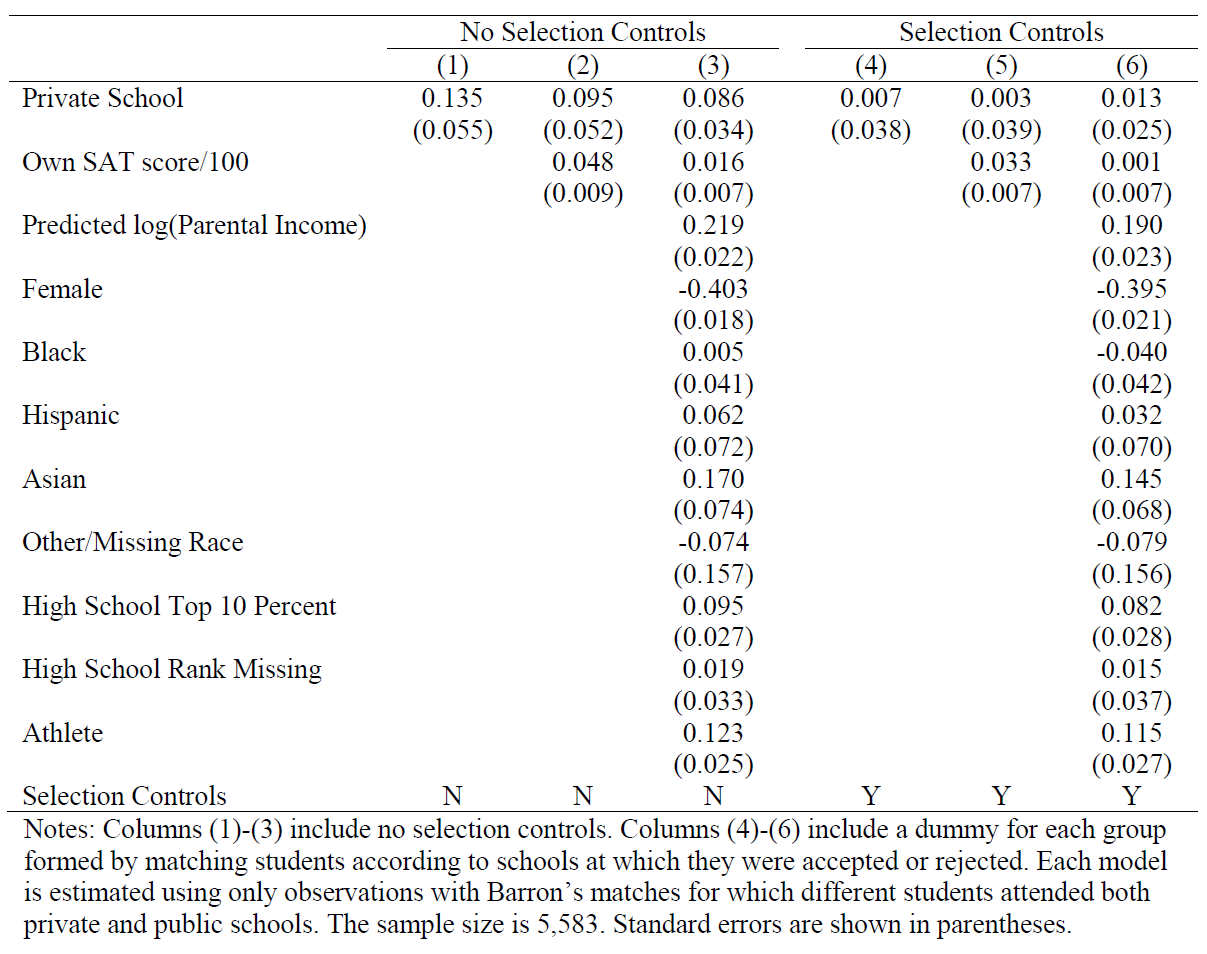
\includegraphics[width=0.9\textwidth]{figures/DK02.png}
		\end{center}
	\end{frame}

	\begin{frame}{Outline}
		\textcolor{red!75!green!50!blue!25!gray}{1. Selection on Observables}$\checkmark$
		\vspace{0.8cm}

		2. Design vs. Outcome Models
		\vspace{0.8cm}

		\textcolor{red!75!green!50!blue!25!gray}{3. Design-Based IV}
	\end{frame}

	\begin{frame}{Why are Multi-Way FE Different?}
		\begin{itemize}
			\item Consider a two-way fixed effect (FE) regression estimated in a panel
				of individuals $i$ observed over time periods $t$:
				\begin{align*}
					y_{it}= \beta x_{it}+ \alpha_{i} + \tau_{t} + \nu_{it}
				\end{align*}\pause{} Q: Can we justify this specification by selection-on-observables?
				\bigskip
				\pause{}

			\item Note that the unit \& time FE controls uniquely identify observations
				\smallskip
				\pause{}
				\begin{itemize}
					\item What would it mean for $x_{it}$ to be as-if-randomly-assigned given
						$(i,t)$?
				\end{itemize}\pause{}
				\bigskip

			\item The auxiliary regression is of $x_{it}$ on two-way FEs (no
				interactions)
				\smallskip
				\begin{itemize}
					\item Is additivity, i.e. $E[x_{it}\mid (i,t)]=\mu_{i} + \gamma_{t}$,
						realistic to impose?
						\smallskip
						\pause{}

					\item Clearly can't make this specification more flexible without ``dummying
						out'' observations (there's no observed variation in $x_{it}$ given
						$(i,t)$)
				\end{itemize}
				\medskip
				\pause{}

			\item We need a different justification for this sort of regression...
		\end{itemize}
	\end{frame}

	\begin{frame}{Two-Way FE as Outcome Modeling}
		\vspace{0.2cm}
		\begin{itemize}
			\item Continue to assume a constant-effects causal model:
				$y_{it}=\beta x_{it}+\varepsilon_{it}$
				\smallskip
				\begin{itemize}
					\item Assume $x_{it}$ is \emph{deterministic} in the set of unit and
						time indicators, $w_{it}$: once I know the unit and period, I know the
						treatment status
						\smallskip

					\item No scope for selection-on-observables
				\end{itemize}
				\bigskip
				\pause{}

			\item Add in a model for untreated potential outcomes:
				$E[\varepsilon_{it}\mid w_{it}]=\alpha_{i} + \tau_{t}$
				\smallskip
				\begin{itemize}
					\item ``Parallel trends'': units with different treatment paths have
						different outcome levels but common outcome changes
				\end{itemize}
				\bigskip
				\pause{}

			\item Putting both models together, we have:
				\begin{align*}
					E[y_{it}\mid x_{it},w_{it}] = \pause{}\beta x_{it}+ E[\varepsilon_{it}\mid w_{it}]=\pause{}\beta x_{it}+\alpha_{i} + \tau_{t}
				\end{align*}\pause{} i.e. the CEF of $y_{it}\mid x_{it},w_{it}$ is
				linear, with a causal coefficient of $\beta$ $\implies$ regression identifies
				it
				\smallskip
				\pause{}
				\begin{itemize}
					\item Logic clearly extends to more than two FEs, time-varying
						controls, unit-specific trends, or any other model for
						$E[\varepsilon\mid w]$
				\end{itemize}
		\end{itemize}
	\end{frame}

	\begin{frame}{Example: Finkelstein (2007)}
		\begin{itemize}
			\item Boiling multi-way FE regression specs down to simpler ``diff-in-diff'
				comparisons can make the content of the outcome model clearer
				\smallskip
				\begin{itemize}
					\item Useful fact: in two periods, $\beta$ in $y_{it}=\beta x_{it}+\alpha
						_{i}+\tau_{t}+\nu_{it}$ is given by the regression of $y_{i,Post}-y_{i,Pre}$
						on $x_{i,Post}-x_{i,Pre}$ (and a constant)
				\end{itemize}
				\medskip
				\pause{}

			\item Finkelstein is interested in estimating market-level effects of health
				insurance coverage, using the 1965 introduction of Medicare
				\smallskip
				\pause{}
				\begin{itemize}
					\item Effectively estimates $y_{it}=\beta x_{it}+\alpha_{i}+\tau_{t}+\nu
						_{it}$ where $x_{it}$ is the share of elderly in market $i$ and year
						$t$ with health insurance
						\smallskip
						\pause{}

					\item Post 1965, $x_{it}=1$ for all markets; previously far from random
				\end{itemize}
				\medskip
				\pause{}

			\item Consider two-period version: equivalent to regressing
				$y_{i,Post}-y_{i,Pre}$ on $x_{i,Post}-x_{i,Pre}=1-x_{i,Pre}$: the pre-Medicare
				uninsured share in $i$
				\smallskip
				\pause{}
				\begin{itemize}
					\item Outcome model: if not for the introduction of Medicare, markets with
						higher/lower uninsured shares would have been on parallel trends
						\smallskip
						\pause{}

					\item Event study version:
						$y_{it}= \alpha_{i} + \tau_{t} + \sum_{s}\beta_{s} (1-x_{i,Pre}) \mathbf{1}
						[t=s] + \nu_{it}$; expect flat pre/post trends if the model is right...
				\end{itemize}
		\end{itemize}
	\end{frame}

	\begin{frame}{Finkelstein Event Study}
		\vspace{-0.1cm}
		\begin{center}
			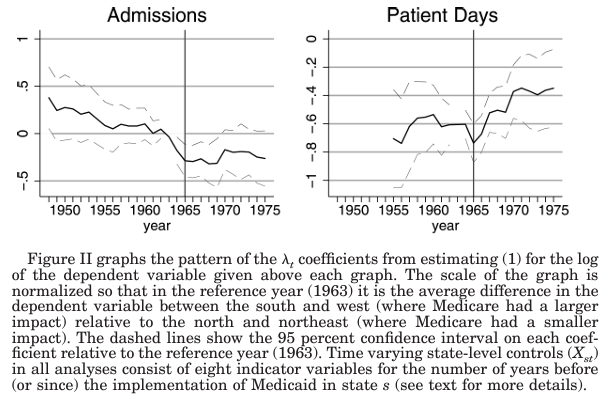
\includegraphics[width=0.9\textwidth]{figures/fink.png}
		\end{center}
	\end{frame}

	\begin{frame}{Different Roles of Controls}
		\begin{itemize}
			\item In a design-based specification, the controls can be understood as
				specifying \emph{which treated/control observations} are valid to compare
				\smallskip
				\begin{itemize}
					\item E.g. private vs. non-private students w/same applications+admissions
						\smallskip
						\pause{}

					\item Think about how the auxiliary regression isolates variation in $x
						_{it}$
				\end{itemize}
				\bigskip
				\pause{}

			\item In an outcome-model-based specification, the controls can be seen as
				specifying \emph{what transformations of the outcomes} are valid to compare
				\smallskip
				\begin{itemize}
					\item E.g. TWFE regressions compare trends in the outcome, allowing the
						outcome levels to be confounded
						\smallskip
						\pause{}

					\item Think about what ``diff-in-diff'' comparisons are underlying the
						spec
				\end{itemize}
				\bigskip
				\pause{}

			\item Both strategies have \emph{ex post} validations (balance tests / pre-trend
				checks), but the \emph{ex ante} case for design is arguably easier to
				make
				\smallskip
				\begin{itemize}
					\item What $\varepsilon_{it}$ model is best? E.g. does parallel trends
						hold in levels or logs?
				\end{itemize}
		\end{itemize}
	\end{frame}

	\begin{frame}{Outline}
		\textcolor{red!75!green!50!blue!25!gray}{1. Selection on Observables}$\checkmark$
		\vspace{0.8cm}

		\textcolor{red!75!green!50!blue!25!gray}{2. Design vs. Outcome Models }$\checkmark$
		\vspace{0.8cm}

		3. Design-Based IV
	\end{frame}

	\begin{frame}{The Simplest IV Story}
		\begin{itemize}
			\item Again start w/constant fx model $y_{i}=\beta x_{i}+\varepsilon_{i}$,
				now $Cov(x_{i},\varepsilon_{i})\neq 0$
				\smallskip
				\begin{itemize}
					\item E.g. $x_{i}$ is enrollment in this class and $y_{i}$ is later
						wages/happiness
						\smallskip

					\item ``Endogeneity'': students in this class have systematically
						higher $\varepsilon_{i}$
				\end{itemize}
				\bigskip
				\pause{}

			\item Imagine the course was ``oversubscribed''; I chose students by
				lottery
				\smallskip
				\begin{itemize}
					\item $z_{i}\in\{0,1\}$ indicates randomized admission to the course
						\smallskip

					\item Randomness + no direct effects of $z_{i}$ on $y_{i}$ implies $Cov
						(z_{i},\varepsilon_{i})=0$
				\end{itemize}
				\bigskip
				\pause{}

			\item Plugging in the model for $\varepsilon_{i}=y_{i}-\beta x_{i}$, we
				have IV identification:
				\begin{align*}
					Cov(z_{i},y_{i}-\beta x_{i})=0\implies \frac{Cov(z_{i},y_{i})}{Cov(z_{i},x_{i})}=\beta
				\end{align*}
				so long as $Cov(z_{i},x_{i})\neq 0$ (``relevance'')
		\end{itemize}
	\end{frame}

	\begin{frame}{Regression ``Endogeneity''}
		\begin{center}
			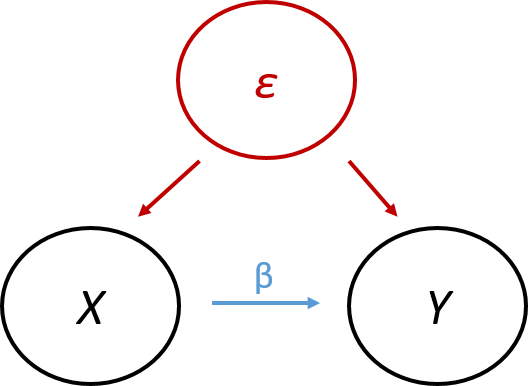
\includegraphics[width=0.5\textwidth]{figures/dag2.png}
		\end{center}
	\end{frame}

	\begin{frame}{Instrument ``Exogeneity'' / ``Validity''}
		\begin{center}
			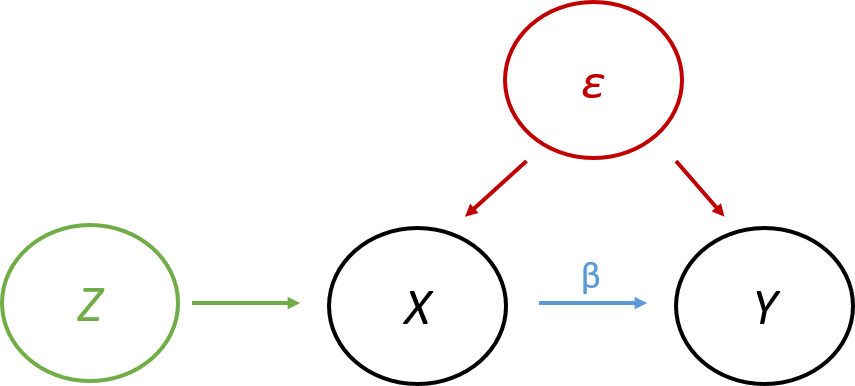
\includegraphics[width=0.9\textwidth]{figures/dag3.png}
		\end{center}
	\end{frame}

	\begin{frame}{Threats to Validity: Instrument Assignment}
		\vspace{0.2cm}

		\begin{center}
			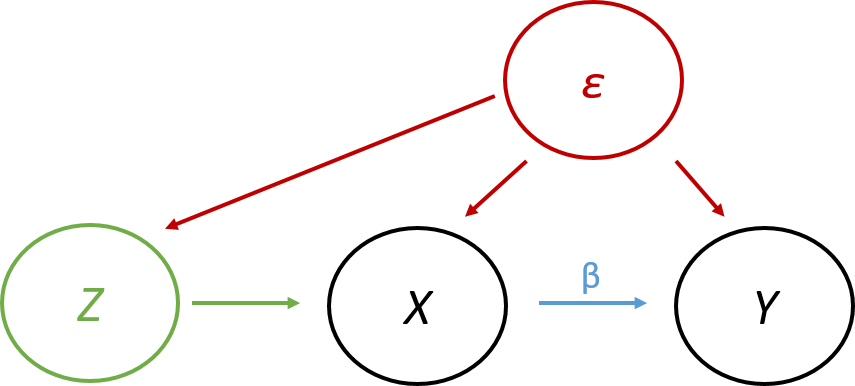
\includegraphics[width=0.9\textwidth]{figures/dag4.png}
		\end{center}
		We will later formalize this as a failure of instrument ``independence''
	\end{frame}

	\begin{frame}{Threats to Validity: Direct Effects}
		\vspace{0.2cm}

		\begin{center}
			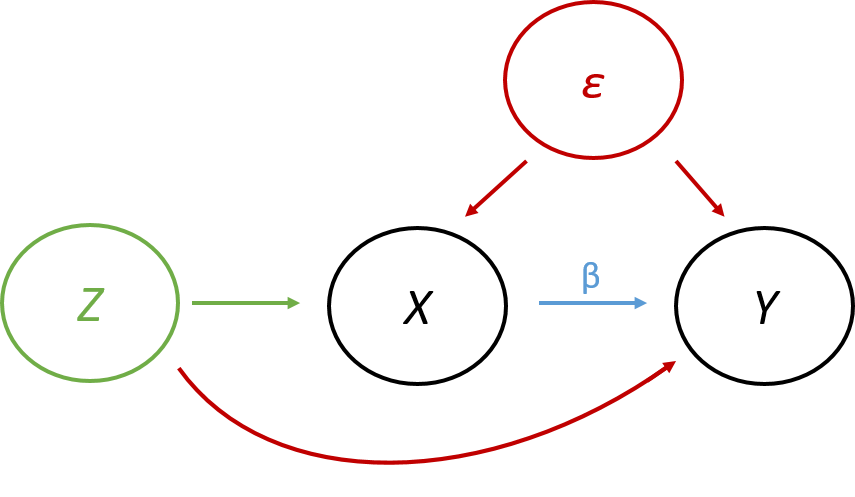
\includegraphics[width=0.9\textwidth]{figures/dag5.png}
		\end{center}
		We will later formalize this as a failure of instrument ``exclusion''
	\end{frame}

	\begin{frame}{Adding Controls and Instruments}
		\begin{itemize}
			\item Basic IV is $\frac{Cov(z_{i},y_{i})}{Cov(z_{i},x_{i})}=\frac{Cov(z_{i},y_{i})/Var(z_{i})}{Cov(z_{i},x_{i})/Var(z_{i})}
				=\rho/\pi$ from the regressions:
				\begin{align*}
					y_{i} & = \kappa + \rho z_{i} + \nu_{i} \hspace{0.2cm}\text{, the ``reduced form''} \\
					x_{i} & = \mu + \pi z_{i} + \eta_{i}\hspace{0.2cm}\text{, the ``first stage'' }
				\end{align*}\pause{}
				\vspace{-0.3cm}

			\item IV with controls works similarly: $\rho/\pi$ from the controlled
				regressions:
				\begin{align*}
					y_{i} & = \kappa + \rho z_{i} + w_{i}^{\prime}\gamma + \nu_{i} \\
					x_{i} & = \mu + \pi z_{i} + w_{i}^{\prime} \gamma + \eta_{i}
				\end{align*}\pause{}
				\vspace{-0.3cm}

			\item Can also have multiple instruments:
				$(\pi^{\prime} w \pi)^{-1}\pi^{\prime} w \rho$ for some $w$
				\smallskip
				\begin{itemize}
					\item $w$ governs how different RF/FS's are weighted together (e.g. 2SLS)
				\end{itemize}
				\medskip
				\pause{}

			\item RF\&FS are the nuclei of IV; the design-based approach starts w/them
		\end{itemize}
	\end{frame}

	\begin{frame}{Bridging the Gap}
		\begin{itemize}
			\item Design-based IV applies the earlier selection-on-observables logic to
				$z_{i}$:
				\smallskip

				\begin{enumerate}
					\item Claim $z_{i}$ is as-good-as-randomly assigned conditional on some
						$w_{i}$
						\smallskip
						\pause{}

					\item Control flexibly for $w_{i}$ such that regressing $z_{i}$ on it estimates
						$E[z_{i}\mid w_{i}]$
				\end{enumerate}
				\bigskip
				\pause{}

			\item This makes both reduced form and first stage regressions causal
				\smallskip
				\pause{}
				\begin{itemize}
					\item As before, best to both tell a clear \emph{ex ante} story about where
						the $z_{i}\mid w_{i}$ variation comes from and validate as-if-random
						assignment \emph{ex post}
				\end{itemize}
				\bigskip
				\pause{}

			\item New twist: have to also argue exclusion in order to interpret RF/FS
				\smallskip
				\begin{itemize}
					\item Can both argue \emph{ex ante} and sometimes test \emph{ex post}:
						e.g. by looking at effects of $z_{i}$ on other plausible treatment channels
				\end{itemize}
		\end{itemize}
	\end{frame}

	\begin{frame}{Example: Abdulkadiroglu et al. (2016)}
		\begin{itemize}
			\item AAHP are interested in the effect of ``takeover'' charter schools:
				ones which convert a low-performing traditional public school (TPS)
				\smallskip
				\begin{itemize}
					\item Lots of evidence of charter effectiveness from admission lotteries,
						but external validity is an open question
				\end{itemize}
				\bigskip
				\pause{}

			\item Reduced-form selection-on-observables strategy: compare students in
				the TPS pre-takeover to others in similarly low-performing TPS
				\smallskip
				\begin{itemize}
					\item Specifically, match each takeover school to a TPS using baseline
						test score performance and control for match cell fixed effects
				\end{itemize}
				\bigskip
				\pause{}

			\item Exclusion: takeovers only affect later test scores via charter
				enrollment
				\smallskip
				\begin{itemize}
					\item Check whether there are takeover effects in the transition (pre-charter)
						year 0; develop a strategy to use these effects to relax exclusion
				\end{itemize}
		\end{itemize}
	\end{frame}

	\begin{frame}{ Abdulkadiroglu et al. Results}
		\begin{center}
			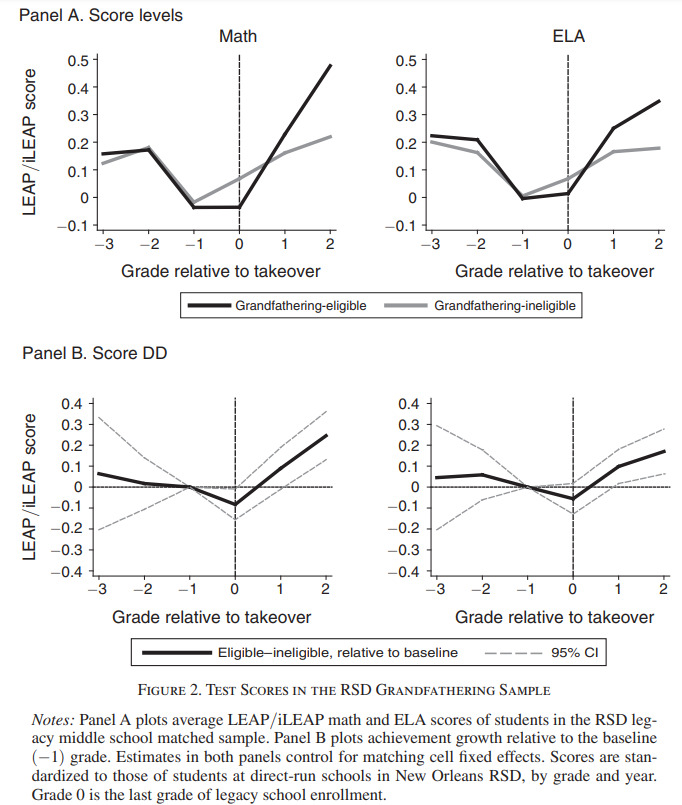
\includegraphics[width=0.6\textwidth]{figures/aahp.png}
		\end{center}
	\end{frame}

	\begin{frame}{Looking Ahead}
		\begin{itemize}
			\item We've now seen the basic design-based logic for regression/IV
				\smallskip
				\begin{itemize}
					\item Main practical takeaway: be clear on what variation in $x_{i}$
						or $z_{i}$ you want to use, and pick controls appropriately for extracting
						it
				\end{itemize}
				\bigskip
				\pause{}

			\item On Wednesday, we'll expand the discussion to other features of
				design
				\smallskip
				\begin{enumerate}
					\item Heterogeneous effects $\implies$ no worries about ``negative weights''
						\smallskip

					\item Inference $\implies$ clearer guidance on how to cluster standard
						errors
				\end{enumerate}
				\bigskip
				\pause{}

			\item Before then, you have the chance to play with a real-world
				application
		\end{itemize}
	\end{frame}
\end{document}
